\begin{figure}[t]
    \centering
    \resizebox{0.98\textwidth}{!}{%
    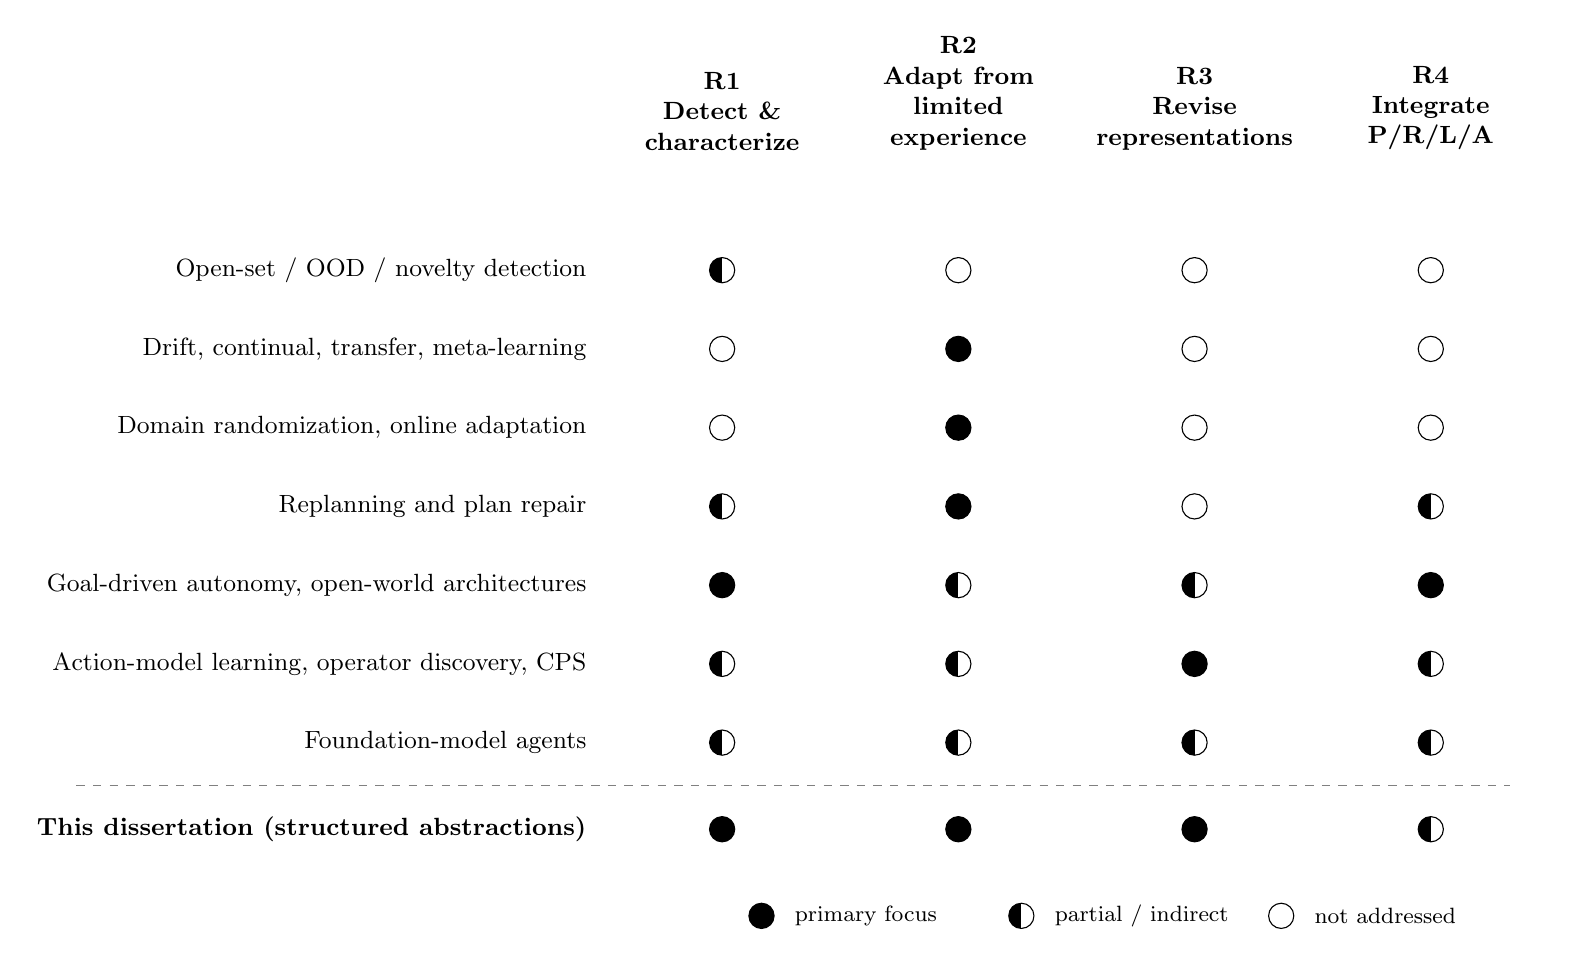
\begin{tikzpicture}[
        rowlabel/.style={anchor=east, align=right, font=\small},
        collabel/.style={anchor=south, align=center, font=\small\bfseries, text width=2.6cm},
        full/.style={circle, draw, fill=black, minimum size=0.32cm, inner sep=0pt},
        half/.style={circle, draw, minimum size=0.32cm, inner sep=0pt, path picture={\fill (path picture bounding box.south west) rectangle (path picture bounding box.north);}},
        none/.style={circle, draw, minimum size=0.32cm, inner sep=0pt},
    ]
    % Column x-positions
    \def\cA{0.0}  % R1 detect & characterize
    \def\cB{3.0}  % R2 adapt from limited experience
    \def\cC{6.0}  % R3 revise representations
    \def\cD{9.0}  % R4 integrate P/R/L/A

    % ===== Column headers =====
    \node[collabel] at (\cA, 0.4) {R1\\ Detect \&\\ characterize};
    \node[collabel] at (\cB, 0.4) {R2\\ Adapt from\\ limited experience};
    \node[collabel] at (\cC, 0.4) {R3\\ Revise\\ representations};
    \node[collabel] at (\cD, 0.4) {R4\\ Integrate\\ P/R/L/A};

    % ===== Rows =====
    % Row 1: Open-set / OOD detection
    \node[rowlabel] at (-1.6, -1.0) {Open-set / OOD / novelty detection};
    \node[half] at (\cA, -1.0) {}; \node[none] at (\cB, -1.0) {}; \node[none] at (\cC, -1.0) {}; \node[none] at (\cD, -1.0) {};

    % Row 2: Re-estimation
    \node[rowlabel] at (-1.6, -2.0) {Drift, continual, transfer, meta-learning};
    \node[none] at (\cA, -2.0) {}; \node[full] at (\cB, -2.0) {}; \node[none] at (\cC, -2.0) {}; \node[none] at (\cD, -2.0) {};

    % Row 3: Robustness / online adaptation
    \node[rowlabel] at (-1.6, -3.0) {Domain randomization, online adaptation};
    \node[none] at (\cA, -3.0) {}; \node[full] at (\cB, -3.0) {}; \node[none] at (\cC, -3.0) {}; \node[none] at (\cD, -3.0) {};

    % Row 4: Replanning / plan repair
    \node[rowlabel] at (-1.6, -4.0) {Replanning and plan repair};
    \node[half] at (\cA, -4.0) {}; \node[full] at (\cB, -4.0) {}; \node[none] at (\cC, -4.0) {}; \node[half] at (\cD, -4.0) {};

    % Row 5: GDA / open-world architectures
    \node[rowlabel] at (-1.6, -5.0) {Goal-driven autonomy, open-world architectures};
    \node[full] at (\cA, -5.0) {}; \node[half] at (\cB, -5.0) {}; \node[half] at (\cC, -5.0) {}; \node[full] at (\cD, -5.0) {};

    % Row 6: Representational extension
    \node[rowlabel] at (-1.6, -6.0) {Action-model learning, operator discovery, CPS};
    \node[half] at (\cA, -6.0) {}; \node[half] at (\cB, -6.0) {}; \node[full] at (\cC, -6.0) {}; \node[half] at (\cD, -6.0) {};

    % Row 7: Foundation-model agents
    \node[rowlabel] at (-1.6, -7.0) {Foundation-model agents};
    \node[half] at (\cA, -7.0) {}; \node[half] at (\cB, -7.0) {}; \node[half] at (\cC, -7.0) {}; \node[half] at (\cD, -7.0) {};

    % Row 8: This dissertation
    \node[rowlabel, font=\small\bfseries] at (-1.6, -8.1) {This dissertation (structured abstractions)};
    \node[full] at (\cA, -8.1) {}; \node[full] at (\cB, -8.1) {}; \node[full] at (\cC, -8.1) {}; \node[half] at (\cD, -8.1) {};

    % Separator above dissertation row
    \draw[gray, dashed] (-8.2, -7.55) -- (10.0, -7.55);

    % ===== Legend =====
    \node[full] at (0.5, -9.2) {};  \node[anchor=west, font=\footnotesize] at (0.8, -9.2) {primary focus};
    \node[half] at (3.8, -9.2) {};  \node[anchor=west, font=\footnotesize] at (4.1, -9.2) {partial / indirect};
    \node[none] at (7.1, -9.2) {};  \node[anchor=west, font=\footnotesize] at (7.4, -9.2) {not addressed};

    \end{tikzpicture}%
    }
    \caption[Method families measured against the requirements for open-world autonomy]{Method families surveyed in this chapter, measured against the four requirements for open-world autonomy identified in \cref{sec:what_is_required}: detecting and characterizing mismatch (R1), adapting from limited experience (R2), revising representations when needed (R3), and integrating perception, reasoning, learning, and action (R4). The assignments reflect the typical emphasis of each family as discussed in the text, not the capabilities of every individual system. The most mature families adapt within fixed representations (R2), while approaches that address representational revision (R3) tend to trade away speed, scope, or generality. This dissertation targets structural adaptation that is fast and localized, using structured abstractions.}
    \label{fig:requirements_coverage}
\end{figure}
